% Options for packages loaded elsewhere
\PassOptionsToPackage{unicode,linktoc=all,pdfwindowui,pdfpagemode=FullScreen}{hyperref}
\PassOptionsToPackage{hyphens}{url}
\PassOptionsToPackage{dvipsnames,svgnames*,x11names*}{xcolor}
%
\documentclass[
  lang=cn,
  11pt,
  scheme=chinese,
  chinesefont=nofont,
  bibstyle=apalike]{elegantbook}
\usepackage{lmodern}
\usepackage{amssymb,amsmath}
\usepackage{ifxetex,ifluatex}
\ifnum 0\ifxetex 1\fi\ifluatex 1\fi=0 % if pdftex
  \usepackage[T1]{fontenc}
  \usepackage[utf8]{inputenc}
  \usepackage{textcomp} % provide euro and other symbols
\else % if luatex or xetex
  \ifxetex
    \usepackage{mathspec}
  \else
    \usepackage{unicode-math}
  \fi
  \defaultfontfeatures{Scale=MatchLowercase}
  \defaultfontfeatures[\rmfamily]{Ligatures=TeX,Scale=1}
\fi
% Use upquote if available, for straight quotes in verbatim environments
\IfFileExists{upquote.sty}{\usepackage{upquote}}{}
\IfFileExists{microtype.sty}{% use microtype if available
  \usepackage[]{microtype}
  \UseMicrotypeSet[protrusion]{basicmath} % disable protrusion for tt fonts
}{}
\makeatletter
\@ifundefined{KOMAClassName}{% if non-KOMA class
  \IfFileExists{parskip.sty}{%
    \usepackage{parskip}
  }{% else
    \setlength{\parindent}{0pt}
    \setlength{\parskip}{6pt plus 2pt minus 1pt}}
}{% if KOMA class
  \KOMAoptions{parskip=half}}
\makeatother
\usepackage{xcolor}
\IfFileExists{xurl.sty}{\usepackage{xurl}}{} % add URL line breaks if available
\IfFileExists{bookmark.sty}{\usepackage{bookmark}}{\usepackage{hyperref}}
\hypersetup{
  pdftitle={Elegant Bookdown Template},
  pdfauthor={黄湘云 \& 叶 飞},
  pdfsubject={基于 elegantbook 文类的 bookdown 模版},
  pdfkeywords={elegantbook, bookdown, pandoc, R},
  colorlinks=true,
  linkcolor=Maroon,
  filecolor=Maroon,
  citecolor=Blue,
  urlcolor=Blue,
  pdfcreator={LaTeX via pandoc}}
\urlstyle{same} % disable monospaced font for URLs
\usepackage{color}
\usepackage{fancyvrb}
\newcommand{\VerbBar}{|}
\newcommand{\VERB}{\Verb[commandchars=\\\{\}]}
\DefineVerbatimEnvironment{Highlighting}{Verbatim}{commandchars=\\\{\}}
% Add ',fontsize=\small' for more characters per line
\usepackage{framed}
\definecolor{shadecolor}{RGB}{248,248,248}
\newenvironment{Shaded}{\begin{snugshade}}{\end{snugshade}}
\newcommand{\AlertTok}[1]{\textcolor[rgb]{0.94,0.16,0.16}{#1}}
\newcommand{\AnnotationTok}[1]{\textcolor[rgb]{0.56,0.35,0.01}{\textbf{\textit{#1}}}}
\newcommand{\AttributeTok}[1]{\textcolor[rgb]{0.77,0.63,0.00}{#1}}
\newcommand{\BaseNTok}[1]{\textcolor[rgb]{0.00,0.00,0.81}{#1}}
\newcommand{\BuiltInTok}[1]{#1}
\newcommand{\CharTok}[1]{\textcolor[rgb]{0.31,0.60,0.02}{#1}}
\newcommand{\CommentTok}[1]{\textcolor[rgb]{0.56,0.35,0.01}{\textit{#1}}}
\newcommand{\CommentVarTok}[1]{\textcolor[rgb]{0.56,0.35,0.01}{\textbf{\textit{#1}}}}
\newcommand{\ConstantTok}[1]{\textcolor[rgb]{0.00,0.00,0.00}{#1}}
\newcommand{\ControlFlowTok}[1]{\textcolor[rgb]{0.13,0.29,0.53}{\textbf{#1}}}
\newcommand{\DataTypeTok}[1]{\textcolor[rgb]{0.13,0.29,0.53}{#1}}
\newcommand{\DecValTok}[1]{\textcolor[rgb]{0.00,0.00,0.81}{#1}}
\newcommand{\DocumentationTok}[1]{\textcolor[rgb]{0.56,0.35,0.01}{\textbf{\textit{#1}}}}
\newcommand{\ErrorTok}[1]{\textcolor[rgb]{0.64,0.00,0.00}{\textbf{#1}}}
\newcommand{\ExtensionTok}[1]{#1}
\newcommand{\FloatTok}[1]{\textcolor[rgb]{0.00,0.00,0.81}{#1}}
\newcommand{\FunctionTok}[1]{\textcolor[rgb]{0.00,0.00,0.00}{#1}}
\newcommand{\ImportTok}[1]{#1}
\newcommand{\InformationTok}[1]{\textcolor[rgb]{0.56,0.35,0.01}{\textbf{\textit{#1}}}}
\newcommand{\KeywordTok}[1]{\textcolor[rgb]{0.13,0.29,0.53}{\textbf{#1}}}
\newcommand{\NormalTok}[1]{#1}
\newcommand{\OperatorTok}[1]{\textcolor[rgb]{0.81,0.36,0.00}{\textbf{#1}}}
\newcommand{\OtherTok}[1]{\textcolor[rgb]{0.56,0.35,0.01}{#1}}
\newcommand{\PreprocessorTok}[1]{\textcolor[rgb]{0.56,0.35,0.01}{\textit{#1}}}
\newcommand{\RegionMarkerTok}[1]{#1}
\newcommand{\SpecialCharTok}[1]{\textcolor[rgb]{0.00,0.00,0.00}{#1}}
\newcommand{\SpecialStringTok}[1]{\textcolor[rgb]{0.31,0.60,0.02}{#1}}
\newcommand{\StringTok}[1]{\textcolor[rgb]{0.31,0.60,0.02}{#1}}
\newcommand{\VariableTok}[1]{\textcolor[rgb]{0.00,0.00,0.00}{#1}}
\newcommand{\VerbatimStringTok}[1]{\textcolor[rgb]{0.31,0.60,0.02}{#1}}
\newcommand{\WarningTok}[1]{\textcolor[rgb]{0.56,0.35,0.01}{\textbf{\textit{#1}}}}
\usepackage{longtable,booktabs}
% Correct order of tables after \paragraph or \subparagraph
\usepackage{etoolbox}
\makeatletter
\patchcmd\longtable{\par}{\if@noskipsec\mbox{}\fi\par}{}{}
\makeatother
% Allow footnotes in longtable head/foot
\IfFileExists{footnotehyper.sty}{\usepackage{footnotehyper}}{\usepackage{footnote}}
\makesavenoteenv{longtable}
\usepackage{graphicx}
\makeatletter
\def\maxwidth{\ifdim\Gin@nat@width>\linewidth\linewidth\else\Gin@nat@width\fi}
\def\maxheight{\ifdim\Gin@nat@height>\textheight\textheight\else\Gin@nat@height\fi}
\makeatother
% Scale images if necessary, so that they will not overflow the page
% margins by default, and it is still possible to overwrite the defaults
% using explicit options in \includegraphics[width, height, ...]{}
\setkeys{Gin}{width=\maxwidth,height=\maxheight,keepaspectratio}
% Set default figure placement to htbp
\makeatletter
\def\fps@figure{htbp}
\makeatother
\setlength{\emergencystretch}{3em} % prevent overfull lines
\providecommand{\tightlist}{%
  \setlength{\itemsep}{0pt}\setlength{\parskip}{0pt}}
\setcounter{secnumdepth}{5}
\institute{A bookdown wrapper for ElegantBook}
\version{ElegantBook 3.11} % 当前使用的 elegantbook 宏包版本
\bioinfo{自定义}{信息}
\extrainfo{Victory won\rq t come to us unless we go to it. --- M. Moore}

% 字体设置
\setCJKmainfont[BoldFont={Adobe Heiti Std},ItalicFont={Adobe Kaiti Std}]{Adobe Song Std} 
\setCJKsansfont[BoldFont={Adobe Heiti Std},ItalicFont={Adobe Heiti Std}]{Adobe Heiti Std} 
\setCJKmonofont[BoldFont={Adobe Heiti Std},ItalicFont={Adobe Heiti Std}]{Adobe Fangsong Std} 

\setCJKfamilyfont{zhsong}{Adobe Song Std}
\setCJKfamilyfont{zhhei}{Adobe Heiti Std} 
\setCJKfamilyfont{zhkai}{Adobe Kaiti Std} 
\setCJKfamilyfont{zhfs}{Adobe Fangsong Std}

\newcommand*{\songti}{\CJKfamily{zhsong}} 
\newcommand*{\heiti}{\CJKfamily{zhhei}} 
\newcommand*{\kaishu}{\CJKfamily{zhkai}} 
\newcommand*{\fangsong}{\CJKfamily{zhfs}}

% 下面如果不注释就准备好 Logo 和封面图片
% \logo{logo-blue.png} % 图片尺寸 1:1
% \cover{cover.jpg} % 图片尺寸 1280 × 1024

% Cancel common factors in Math 
\usepackage[makeroom]{cancel}

\usepackage[export]{adjustbox} %Needed for max width
%\patchcmd{<command>}{<code to replace>}{<code>}{<success>}{<failure>}
%The following codes add max dimension option to includegraphics
%Gin@ii is from graphicx package and looks for a second optional argument
\expandafter\patchcmd\csname Gin@ii\endcsname 
{\setkeys{Gin}{#1}}
{\setkeys{Gin}{max width=\textwidth, max height=.5\textwidth,keepaspectratio,#1}}
{}
{}

%% 自定义块
\definecolor{colortip}{RGB}{81,183,73}
\definecolor{colornote}{RGB}{251,188,5}
\definecolor{colorwarn}{RGB}{255,83,59}
\definecolor{colorinfo}{RGB}{204,204,204}

\newtcolorbox{rmdtip}{
  colback=white, % 背景色
  colframe=colortip, % 边框色
  coltext=black, % 文本色
  leftrule=1mm,
  rightrule=.25mm,
  bottomrule=.25mm,
  toprule=.25mm,
  boxsep=1pt, % 文字和边框的空隙
  arc=1pt % 圆角
}

\newtcolorbox{rmdnote}{
  colback=white, % 背景色
  colframe=colornote, % 边框色
  coltext=black, % 文本色
  leftrule=1mm,
  rightrule=.25mm,
  bottomrule=.25mm,
  toprule=.25mm,
  boxsep=1pt, % 文字和边框的空隙
  arc=1pt % 圆角
}

\newtcolorbox{rmdwarn}{
  colback=white, % 背景色
  colframe=colorwarn, % 边框色
  coltext=black, % 文本色
  leftrule=1mm,
  rightrule=.25mm,
  bottomrule=.25mm,
  toprule=.25mm,
  boxsep=1pt, % 文字和边框的空隙
  arc=1pt % 圆角
}

\newtcolorbox{rmdinfo}{
  colback=white, % 背景色
  colframe=colorinfo, % 边框色
  coltext=black, % 文本色
  leftrule=1mm,
  rightrule=.25mm,
  bottomrule=.25mm,
  toprule=.25mm,
  boxsep=1pt, % 文字和边框的空隙
  arc=1pt % 圆角
}

\frontmatter
\usepackage[lotdepth=2, lofdepth=2]{subfig}
\usepackage[scale=0.85]{sourcecodepro}
\newlength{\cslhangindent}
\setlength{\cslhangindent}{1.5em}
\newenvironment{cslreferences}%
  {\setlength{\parindent}{0pt}%
  \everypar{\setlength{\hangindent}{\cslhangindent}}\ignorespaces}%
  {\par}

\title{Elegant Bookdown Template}
\usepackage{etoolbox}
\makeatletter
\providecommand{\subtitle}[1]{% add subtitle to \maketitle
  \apptocmd{\@title}{\par {\large #1 \par}}{}{}
}
\makeatother
\subtitle{优雅的 Bookdown 书籍模版}
\author{黄湘云 \& 叶 飞}
\date{2020-05-07}

\let\BeginKnitrBlock\begin \let\EndKnitrBlock\end
\begin{document}
\maketitle

{
\hypersetup{linkcolor=Maroon}
\setcounter{tocdepth}{2}
\tableofcontents
}
\listoftables
\listoffigures
\mainmatter

\hypertarget{welcome}{%
\chapter{欢迎}\label{welcome}}

\begin{quote}
A Markdown-formatted document should be publishable as-is, as plain text, without looking like it's been marked up with tags or formatting instructions.

\hspace*{\fill} --- John Gruber
\end{quote}

这是一份 R Markodwn 文档。 Markdown 提供一种简洁的格式语法,用来生成 HTML、PDF 和 MS Word 文档。

当你点击 \textbf{Knit} 按钮时,就会生成一份包含正文和代码执行结果的文档。你可以像这样嵌入 R 代码块:

\begin{Shaded}
\begin{Highlighting}[]
\KeywordTok{summary}\NormalTok{(cars)}
\end{Highlighting}
\end{Shaded}

\begin{verbatim}
##      speed           dist       
##  Min.   : 4.0   Min.   :  2.00  
##  1st Qu.:12.0   1st Qu.: 26.00  
##  Median :15.0   Median : 36.00  
##  Mean   :15.4   Mean   : 42.98  
##  3rd Qu.:19.0   3rd Qu.: 56.00  
##  Max.   :25.0   Max.   :120.00
\end{verbatim}

\hypertarget{pr}{%
\section{如何参与改进}\label{pr}}

改进原则

\begin{enumerate}
\def\labelenumi{\arabic{enumi}.}

\item
  不要引入新的 LaTeX 宏包,在我看来,上游 \href{https://github.com/ElegantLaTeX/ElegantBook}{ElegantBook} 使用的宏包已经足够多了,详见 \url{https://d.cosx.org/d/421349-latex/2}
\item
  书籍风格尽可能简洁,本人信奉 simple is better
\item
  不要自定义 Pandoc's LaTeX 模版,Pandoc 内建的模版已经功能很全面了,下游的 R Markdown 生态已经甩掉了自己造的大量 LaTeX 模版。为保持与下游的完美兼容,也为了更加轻量地输出多种文档格式,也尽可能多地保持多种输出格式的风格一致。
\item
  本书输出格式目标是 HTML/PDF/EPUB,可以推动上游优化 Pandoc 模版或者 \href{https://github.com/ElegantLaTeX/ElegantBook}{ElegantBook} 模版
\end{enumerate}

\hypertarget{session-info}{%
\section{运行环境}\label{session-info}}

\begin{Shaded}
\begin{Highlighting}[]
\NormalTok{xfun}\OperatorTok{::}\KeywordTok{session\_info}\NormalTok{(}\KeywordTok{c}\NormalTok{(}\StringTok{"rmarkdown"}\NormalTok{, }\StringTok{"bookdown"}\NormalTok{, }\StringTok{"knitr"}\NormalTok{), }\DataTypeTok{dependencies =} \OtherTok{FALSE}\NormalTok{)}
\end{Highlighting}
\end{Shaded}

\begin{verbatim}
## R version 4.0.0 (2020-04-24)
## Platform: x86_64-pc-linux-gnu (64-bit)
## Running under: Ubuntu 16.04.6 LTS
## 
## Locale:
##   LC_CTYPE=en_US.UTF-8       LC_NUMERIC=C              
##   LC_TIME=en_US.UTF-8        LC_COLLATE=en_US.UTF-8    
##   LC_MONETARY=en_US.UTF-8    LC_MESSAGES=en_US.UTF-8   
##   LC_PAPER=en_US.UTF-8       LC_NAME=C                 
##   LC_ADDRESS=C               LC_TELEPHONE=C            
##   LC_MEASUREMENT=en_US.UTF-8 LC_IDENTIFICATION=C       
## 
## Package version:
##   bookdown_0.18 knitr_1.28    rmarkdown_2.1
## 
## Pandoc version: 2.9.2
\end{verbatim}

文武线

\begin{Shaded}
\begin{Highlighting}[]
\KeywordTok{ruler}\NormalTok{()}
\end{Highlighting}
\end{Shaded}

\begin{verbatim}
----+----1----+----2----+----3----+----4----+----5----+----6----+----
123456789012345678901234567890123456789012345678901234567890123456789
\end{verbatim}

\hypertarget{pandoc}{%
\section{Pandoc}\label{pandoc}}

Pandoc 自诞生以来已历 15 个春秋,Github 星级 18.5k,而日常使用的 Hive 不过区区 3k。Pandoc 现已被各大 Linux 发行版(如 CentOS/Ubuntu 等)收录。下面给出一个使用 Pandoc 的简单例子

\begin{Shaded}
\begin{Highlighting}[]
\BuiltInTok{echo} \StringTok{"hello, world!"} \OperatorTok{\textgreater{}}\NormalTok{ note.md}
\ExtensionTok{pandoc}\NormalTok{ note.md {-}s {-}o note.tex }\CommentTok{\# markdown 文本转化为 tex 文本}
\ExtensionTok{pandoc}\NormalTok{ note.md {-}o note.pdf    }\CommentTok{\# markdown 文本转化为 pdf 文档}
\ExtensionTok{pandoc}\NormalTok{ note.md {-}o note.html   }\CommentTok{\# markdown 文本转化为 html 文档}
\end{Highlighting}
\end{Shaded}

Pandoc 支持数十种文档输出格式,更多命令参数说明见 \url{https://pandoc.org/MANUAL.html}。可不可以不要 R,也不要 R Markdown 呢?当然可以,详见 \url{https://github.com/annProg/PanBook},基于 Pandoc's Markdown 实现一次写作,多样输出!

\hypertarget{theorem-block}{%
\section{已有 Block}\label{theorem-block}}

\BeginKnitrBlock{lemma}{}{}
\protect\hypertarget{lem:chf-pdf}{}{\label{lem:chf-pdf} }For any two random variables \(X_1\), \(X_2\), they both have the same probability distribution if and only if \[\varphi _{X_1}(t)=\varphi _{X_2}(t)\]
\EndKnitrBlock{lemma}

\BeginKnitrBlock{theorem}{}{}
\protect\hypertarget{thm:chf-sum}{}{\label{thm:chf-sum} }If \(X_1\), \ldots, \(X_n\) are independent random variables, and \(a_1\), \ldots, \(a_n\) are some constants, then the characteristic function of the linear combination \(S_n=\sum_{i=1}^na_iX_i\) is \[\varphi _{S_{n}}(t)=\prod_{i=1}^n\varphi _{X_i}(a_{i}t)=\varphi _{X_{1}}(a_{1}t)\cdots \varphi _{X_{n}}(a_{n}t)\]
\EndKnitrBlock{theorem}

\BeginKnitrBlock{proposition}{}{}
\protect\hypertarget{prp:unnamed-chunk-5}{}{\label{prp:unnamed-chunk-5} }The distribution of the sum of independent Poisson random variables \(X_i \sim \mathrm{Pois}(\lambda_i),\: i=1,2,\cdots,n\) is \(\mathrm{Pois}(\sum_{i=1}^n\lambda_i)\).
\EndKnitrBlock{proposition}

\BeginKnitrBlock{proof}
\iffalse{} {证明 } \fi{}The characteristic function of \(X\sim\mathrm{Pois}(\lambda)\) is \(\varphi _{X}(t)=e^{\lambda (e^{it}-1)}\). Let \(P_n=\sum_{i=1}^nX_i\). We know from Theorem \ref{thm:chf-sum} that \begin{equation*}
\begin{split}
\varphi _{P_{n}}(t) & =\prod_{i=1}^n\varphi _{X_i}(t) \\
& =\prod_{i=1}^n e^{\lambda_i (e^{it}-1)} \\
& = e^{\sum_{i=1}^n \lambda_i (e^{it}-1)}
\end{split}
\end{equation*} This is the characteristic function of a Poisson random variable with the parameter \(\lambda=\sum_{i=1}^n \lambda_i\). From Lemma \ref{lem:chf-pdf}, we know the distribution of \(P_n\) is \(\mathrm{Pois}(\sum_{i=1}^n\lambda_i)\).
\EndKnitrBlock{proof}

\BeginKnitrBlock{remark}
\iffalse{} {注 } \fi{}In some cases, it is very convenient and easy to figure out the distribution of the sum of independent random variables using characteristic functions.
\EndKnitrBlock{remark}

\BeginKnitrBlock{corollary}{}{}
\protect\hypertarget{cor:unnamed-chunk-8}{}{\label{cor:unnamed-chunk-8} }The characteristic function of the sum of two independent random variables \(X_1\) and \(X_2\) is the product of characteristic functions of \(X_1\) and \(X_2\), i.e., \[\varphi _{X_1+X_2}(t)=\varphi _{X_1}(t) \varphi _{X_2}(t)\]
\EndKnitrBlock{corollary}

\BeginKnitrBlock{exercise}[Characteristic Function of the Sample Mean]
\protect\hypertarget{exr:unnamed-chunk-9}{}{\label{exr:unnamed-chunk-9} \iffalse (Characteristic Function of the Sample Mean) \fi{} }Let \(\bar{X}=\sum_{i=1}^n \frac{1}{n} X_i\) be the sample mean of \(n\) independent and identically distributed random variables, each with characteristic function \(\varphi _{X}\). Compute the characteristic function of \(\bar{X}\).
\EndKnitrBlock{exercise}

\BeginKnitrBlock{solution}
\iffalse{} {解 } \fi{}Applying Theorem \ref{thm:chf-sum}, we have \[\varphi _{\bar{X}}(t)=\prod_{i=1}^n \varphi _{X_i}\left(\frac{t}{n}\right)=\left[\varphi _{X}\left(\frac{t}{n}\right)\right]^n.\]
\EndKnitrBlock{solution}

\hypertarget{math-formular}{%
\section{数学公式}\label{math-formular}}

数学公式加粗可能是最常见的需求之一, \textbf{elegantbook} 宏包提供的文类 \texttt{elegantbook.cls} 已经调用了 \textbf{bm} 宏包\footnote{\url{https://github.com/ElegantLaTeX/ElegantBook/blob/6ab10beda81252f0b478e05fa926199301347e4a/elegantbook.cls\#L884}}。有了 \textbf{bm} 宏包,就可以使用 \textbf{bm} 宏包提供的 \texttt{\textbackslash{}bm\{\}} 命令,而不需要调 \texttt{\textbackslash{}boldsymbol\{\}} 加粗希腊字母,如将 \(\alpha\) (正常)加粗为 \(\bm{\alpha}\)(粗体)。为了在 HTML 网页中显示加粗效果,则还不够,默认情况下, MathJax 是不认识 \texttt{\textbackslash{}bm\{\}} 命令的,所以需要在 \texttt{header.html} 自定义 \texttt{\textbackslash{}bm\{\}} 命令:

\begin{Shaded}
\begin{Highlighting}[]
\KeywordTok{\textless{}script}\OtherTok{ type=}\StringTok{"text/x{-}mathjax{-}config"}\KeywordTok{\textgreater{}}
\NormalTok{    MathJax}\OperatorTok{.}\AttributeTok{Hub}\OperatorTok{.}\FunctionTok{Config}\NormalTok{(\{}
      \DataTypeTok{TeX}\OperatorTok{:}\NormalTok{ \{}
        \DataTypeTok{Macros}\OperatorTok{:}\NormalTok{ \{}
          \DataTypeTok{bm}\OperatorTok{:}\NormalTok{ [}\StringTok{"\{}\SpecialCharTok{\textbackslash{}\textbackslash{}}\StringTok{boldsymbol \#1\}"}\OperatorTok{,}\DecValTok{1}\NormalTok{]}\OperatorTok{,}
\NormalTok{        \}}
\NormalTok{      \}}
\NormalTok{    \})}\OperatorTok{;}
\KeywordTok{\textless{}/script\textgreater{}}
\end{Highlighting}
\end{Shaded}

进一步地,使用常用的 3 个取消符号 \(\bcancel{///}\) 需要在 \texttt{header.html} 添加 JS 库 \texttt{cancel.js},

\begin{Shaded}
\begin{Highlighting}[]
\KeywordTok{\textless{}script}\OtherTok{ type=}\StringTok{"text/x{-}mathjax{-}config"}\KeywordTok{\textgreater{}}
\NormalTok{    MathJax}\OperatorTok{.}\AttributeTok{Hub}\OperatorTok{.}\FunctionTok{Config}\NormalTok{(\{}
      \DataTypeTok{TeX}\OperatorTok{:}\NormalTok{ \{}
        \DataTypeTok{Macros}\OperatorTok{:}\NormalTok{ \{}
          \DataTypeTok{bm}\OperatorTok{:}\NormalTok{ [}\StringTok{"\{}\SpecialCharTok{\textbackslash{}\textbackslash{}}\StringTok{boldsymbol \#1\}"}\OperatorTok{,}\DecValTok{1}\NormalTok{]}\OperatorTok{,}
\NormalTok{        \}}\OperatorTok{,}
        \DataTypeTok{extensions}\OperatorTok{:}\NormalTok{ [}\StringTok{"cancel.js"}\NormalTok{]}
\NormalTok{      \}}
\NormalTok{    \})}\OperatorTok{;}
\KeywordTok{\textless{}/script\textgreater{}}
\end{Highlighting}
\end{Shaded}

并在 preamble.tex 文件中添加一行代码加载 \textbf{cancel} 宏包

\begin{Shaded}
\begin{Highlighting}[]
\BuiltInTok{\textbackslash{}usepackage}\NormalTok{[makeroom]\{}\ExtensionTok{cancel}\NormalTok{\}}
\end{Highlighting}
\end{Shaded}

\hypertarget{custom-block}{%
\section{自定义 block}\label{custom-block}}

基于 Pandoc 自定义 block 是一件很有意思的事情,目前不想让模版过于复杂,仅给出几个最常用的例子。如何自定义可以去看谢益辉的新书 \href{https://bookdown.org/yihui/rmarkdown-cookbook/}{R Markdown Cookbook}\footnote{截止 07 May, 2020 该书尚未出版,自定义 block 的章节见 \url{https://bookdown.org/yihui/rmarkdown-cookbook/custom-blocks.html}}

\textcolor{red}{\textbf{TODO: }{要做的还有很多}}

\begin{rmdwarn}\textcolor[RGB]{255,83,59}{\Large\textbf{警告}}

这是警告

\end{rmdwarn}

\begin{rmdtip}\textcolor[RGB]{81,183,73}{\Large\textbf{提示}}

这是提示

\end{rmdtip}

\begin{rmdnote}\textcolor[RGB]{251,188,5}{\Large\textbf{注意}}

这是注意

\end{rmdnote}

\begin{rmdinfo}

普通说明

\end{rmdinfo}

\hypertarget{intro}{%
\chapter{Introduction}\label{intro}}

You can label chapter and section titles using \texttt{\{\#label\}} after them, e.g., we can reference Chapter \ref{intro}. If you do not manually label them, there will be automatic labels anyway, e.g., Chapter \ref{methods}.

Figures and tables with captions will be placed in \texttt{figure} and \texttt{table} environments, respectively.

\begin{Shaded}
\begin{Highlighting}[]
\KeywordTok{par}\NormalTok{(}\DataTypeTok{mar =} \KeywordTok{c}\NormalTok{(}\DecValTok{4}\NormalTok{, }\DecValTok{4}\NormalTok{, }\FloatTok{.1}\NormalTok{, }\FloatTok{.1}\NormalTok{))}
\KeywordTok{plot}\NormalTok{(pressure, }\DataTypeTok{type =} \StringTok{\textquotesingle{}b\textquotesingle{}}\NormalTok{, }\DataTypeTok{pch =} \DecValTok{19}\NormalTok{)}
\end{Highlighting}
\end{Shaded}

\begin{figure}

{\centering 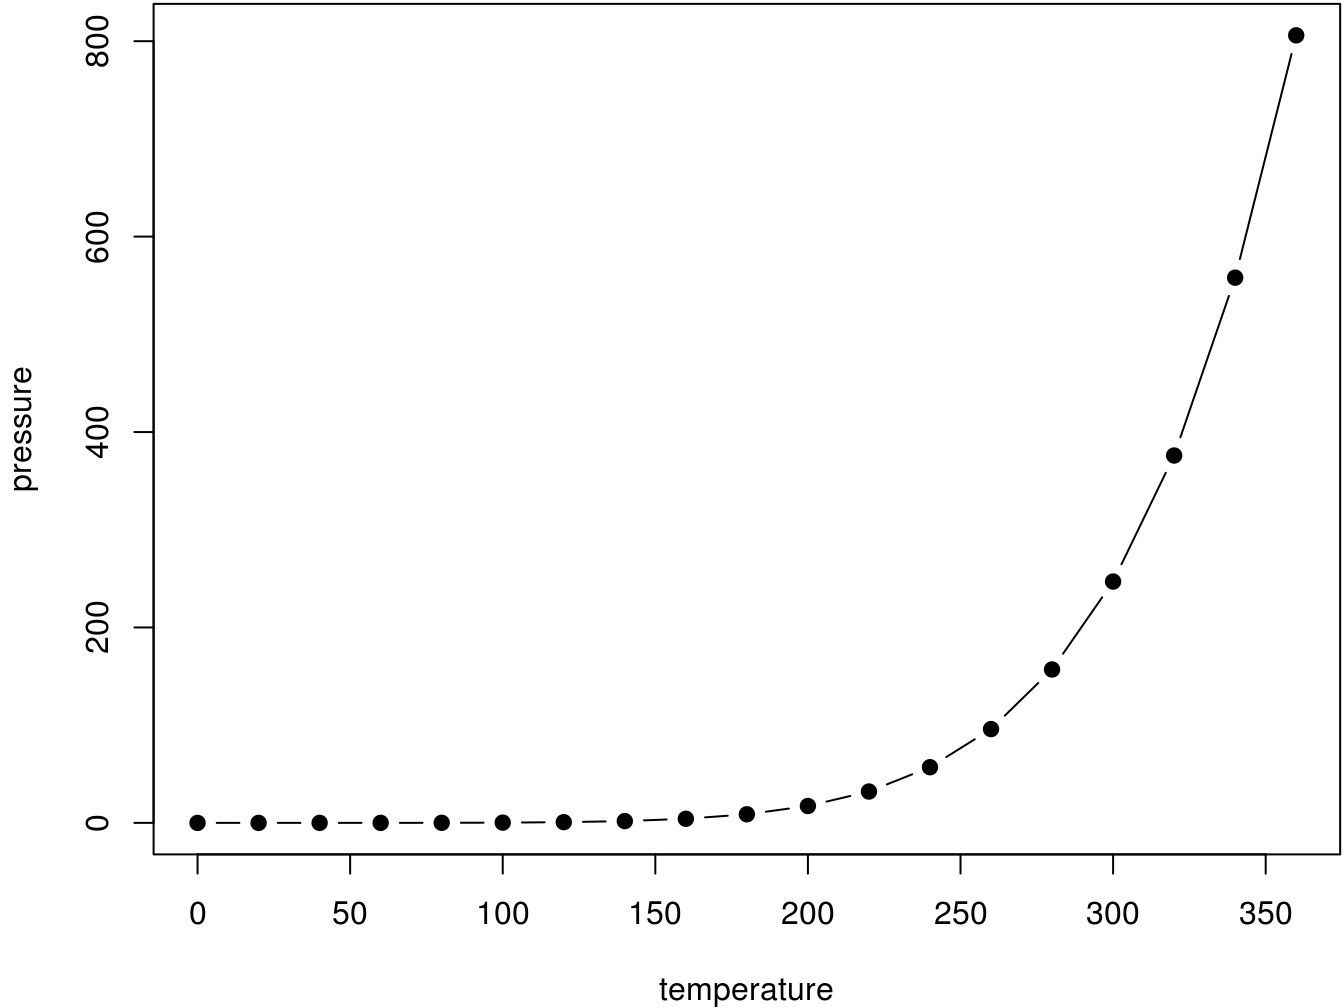
\includegraphics[width=0.8\linewidth]{01-intro_files/figure-latex/nice-fig-1} 

}

\caption{Here is a nice figure!}\label{fig:nice-fig}
\end{figure}

Reference a figure by its code chunk label with the \texttt{fig:} prefix, e.g., see Figure \ref{fig:nice-fig}. Similarly, you can reference tables generated from \texttt{knitr::kable()}, e.g., see Table \ref{tab:nice-tab}.

\begin{Shaded}
\begin{Highlighting}[]
\NormalTok{knitr}\OperatorTok{::}\KeywordTok{kable}\NormalTok{(}
  \KeywordTok{head}\NormalTok{(iris, }\DecValTok{20}\NormalTok{), }\DataTypeTok{caption =} \StringTok{\textquotesingle{}Here is a nice table!\textquotesingle{}}\NormalTok{,}
  \DataTypeTok{booktabs =} \OtherTok{TRUE}
\NormalTok{)}
\end{Highlighting}
\end{Shaded}

\begin{longtable}[]{@{}rrrrl@{}}
\caption{\label{tab:nice-tab}Here is a nice table!}\tabularnewline
\toprule
Sepal.Length & Sepal.Width & Petal.Length & Petal.Width & Species\tabularnewline
\midrule
\endfirsthead
\toprule
Sepal.Length & Sepal.Width & Petal.Length & Petal.Width & Species\tabularnewline
\midrule
\endhead
5.1 & 3.5 & 1.4 & 0.2 & setosa\tabularnewline
4.9 & 3.0 & 1.4 & 0.2 & setosa\tabularnewline
4.7 & 3.2 & 1.3 & 0.2 & setosa\tabularnewline
4.6 & 3.1 & 1.5 & 0.2 & setosa\tabularnewline
5.0 & 3.6 & 1.4 & 0.2 & setosa\tabularnewline
5.4 & 3.9 & 1.7 & 0.4 & setosa\tabularnewline
4.6 & 3.4 & 1.4 & 0.3 & setosa\tabularnewline
5.0 & 3.4 & 1.5 & 0.2 & setosa\tabularnewline
4.4 & 2.9 & 1.4 & 0.2 & setosa\tabularnewline
4.9 & 3.1 & 1.5 & 0.1 & setosa\tabularnewline
5.4 & 3.7 & 1.5 & 0.2 & setosa\tabularnewline
4.8 & 3.4 & 1.6 & 0.2 & setosa\tabularnewline
4.8 & 3.0 & 1.4 & 0.1 & setosa\tabularnewline
4.3 & 3.0 & 1.1 & 0.1 & setosa\tabularnewline
5.8 & 4.0 & 1.2 & 0.2 & setosa\tabularnewline
5.7 & 4.4 & 1.5 & 0.4 & setosa\tabularnewline
5.4 & 3.9 & 1.3 & 0.4 & setosa\tabularnewline
5.1 & 3.5 & 1.4 & 0.3 & setosa\tabularnewline
5.7 & 3.8 & 1.7 & 0.3 & setosa\tabularnewline
5.1 & 3.8 & 1.5 & 0.3 & setosa\tabularnewline
\bottomrule
\end{longtable}

You can write citations, too. For example, we are using the \textbf{bookdown} package (Xie \protect\hyperlink{ref-R-bookdown}{2020}\protect\hyperlink{ref-R-bookdown}{a}) in this sample book, which was built on top of R Markdown and \textbf{knitr} (Xie \protect\hyperlink{ref-xie2015}{2015}\protect\hyperlink{ref-xie2015}{a}).

\hypertarget{literature}{%
\chapter{Literature}\label{literature}}

Here is a review of existing methods.

\hypertarget{methods}{%
\chapter{Methods}\label{methods}}

We describe our methods in this chapter.

\hypertarget{applications}{%
\chapter{Applications}\label{applications}}

Some \emph{significant} applications are demonstrated in this chapter.

\hypertarget{example-one}{%
\section{Example one}\label{example-one}}

\hypertarget{example-two}{%
\section{Example two}\label{example-two}}

\hypertarget{final-words}{%
\chapter{Final Words}\label{final-words}}

We have finished a nice book.

\hypertarget{appendix}{%
\appendix}


\hypertarget{r-markdown}{%
\chapter{R Markdown}\label{r-markdown}}

This is an R Markdown document. Markdown is a simple formatting syntax for authoring HTML, PDF, and MS Word documents. For more details on using R Markdown see \url{http://rmarkdown.rstudio.com}.

When you click the \textbf{Knit} button a document will be generated that includes both content as well as the output of any embedded R code chunks within the document. You can embed an R code chunk like this:

\begin{Shaded}
\begin{Highlighting}[]
\KeywordTok{summary}\NormalTok{(cars)}
\end{Highlighting}
\end{Shaded}

\begin{verbatim}
##      speed           dist       
##  Min.   : 4.0   Min.   :  2.00  
##  1st Qu.:12.0   1st Qu.: 26.00  
##  Median :15.0   Median : 36.00  
##  Mean   :15.4   Mean   : 42.98  
##  3rd Qu.:19.0   3rd Qu.: 56.00  
##  Max.   :25.0   Max.   :120.00
\end{verbatim}

\hypertarget{including-plots}{%
\section{Including Plots}\label{including-plots}}

You can also embed plots, for example:

\begin{Shaded}
\begin{Highlighting}[]
\KeywordTok{par}\NormalTok{(}\DataTypeTok{mar =} \KeywordTok{c}\NormalTok{(}\DecValTok{4}\NormalTok{, }\DecValTok{4}\NormalTok{, }\FloatTok{.1}\NormalTok{, }\FloatTok{.1}\NormalTok{))}
\KeywordTok{plot}\NormalTok{(pressure)}
\end{Highlighting}
\end{Shaded}

\begin{figure}

{\centering 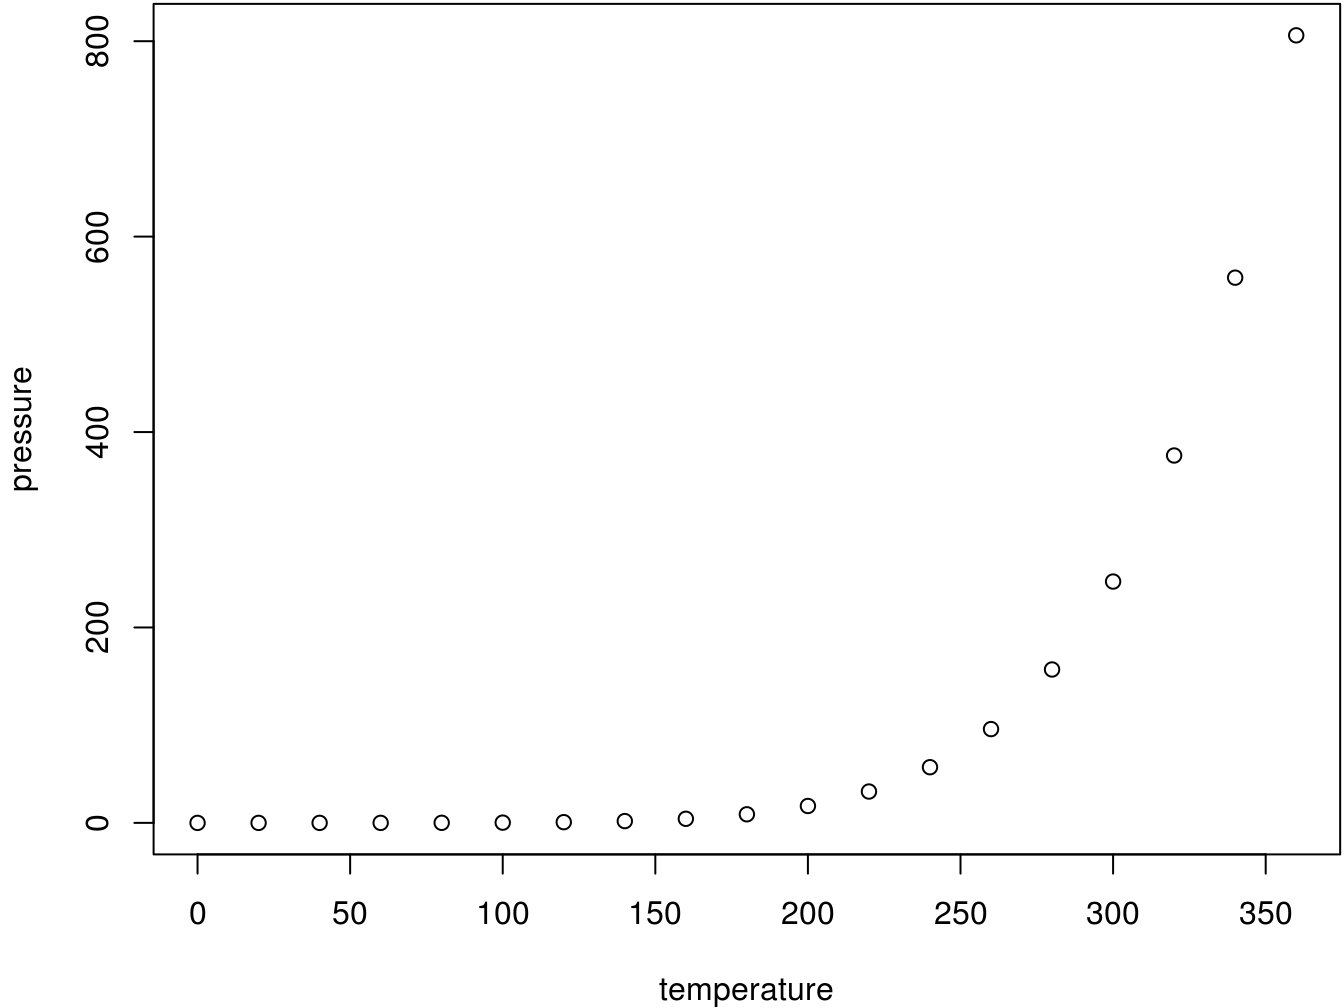
\includegraphics[width=0.8\linewidth]{07-appendix_files/figure-latex/nice-fig-02-1} 

}

\caption{Here is another nice figure!}\label{fig:nice-fig-02}
\end{figure}

Note that the \texttt{echo\ =\ FALSE} parameter was added to the code chunk to prevent printing of the R code that generated the plot.

\hypertarget{References}{%
\chapter*{参考文献}\label{References}}
\addcontentsline{toc}{chapter}{参考文献}

\hypertarget{refs}{}
\begin{cslreferences}
\leavevmode\hypertarget{ref-R-rmarkdown}{}%
Allaire, JJ, Yihui Xie, Jonathan McPherson, Javier Luraschi, Kevin Ushey, Aron Atkins, Hadley Wickham, Joe Cheng, Winston Chang, and Richard Iannone. 2020. \emph{Rmarkdown: Dynamic Documents for R}. \url{https://CRAN.R-project.org/package=rmarkdown}.

\leavevmode\hypertarget{ref-R-base}{}%
R Core Team. 2020. \emph{R: A Language and Environment for Statistical Computing}. Vienna, Austria: R Foundation for Statistical Computing. \url{https://www.R-project.org/}.

\leavevmode\hypertarget{ref-knitr2014}{}%
Xie, Yihui. 2014. ``Knitr: A Comprehensive Tool for Reproducible Research in R.'' In \emph{Implementing Reproducible Computational Research}, edited by Victoria Stodden, Friedrich Leisch, and Roger D. Peng. Chapman; Hall/CRC. \url{http://www.crcpress.com/product/isbn/9781466561595}.

\leavevmode\hypertarget{ref-xie2015}{}%
---------. 2015a. \emph{Dynamic Documents with R and Knitr}. 2nd ed. Boca Raton, Florida: Chapman; Hall/CRC. \url{http://yihui.name/knitr/}.

\leavevmode\hypertarget{ref-knitr2015}{}%
---------. 2015b. \emph{Dynamic Documents with R and Knitr}. 2nd ed. Boca Raton, Florida: Chapman; Hall/CRC. \url{https://yihui.org/knitr/}.

\leavevmode\hypertarget{ref-bookdown2016}{}%
---------. 2016. \emph{Bookdown: Authoring Books and Technical Documents with R Markdown}. Boca Raton, Florida: Chapman; Hall/CRC. \url{https://github.com/rstudio/bookdown}.

\leavevmode\hypertarget{ref-R-bookdown}{}%
---------. 2020a. \emph{Bookdown: Authoring Books and Technical Documents with R Markdown}. \url{https://CRAN.R-project.org/package=bookdown}.

\leavevmode\hypertarget{ref-R-knitr}{}%
---------. 2020b. \emph{Knitr: A General-Purpose Package for Dynamic Report Generation in R}. \url{https://CRAN.R-project.org/package=knitr}.

\leavevmode\hypertarget{ref-rmarkdown2018}{}%
Xie, Yihui, J. J. Allaire, and Garrett Grolemund. 2018. \emph{R Markdown: The Definitive Guide}. Boca Raton, Florida: Chapman; Hall/CRC. \url{https://bookdown.org/yihui/rmarkdown}.
\end{cslreferences}

\end{document}
